\documentclass{beamer}
\usepackage{graphicx}
\usepackage{calc}

\graphicspath{{../images/},{tmp/}}
%\usetheme{shadow}
\usetheme{Singapore}
\useoutertheme{infolines}
\usecolortheme{seahorse}
\useinnertheme[shadow]{rounded}
\setbeamercolor{block title}{bg=black!10!white}

\usepackage{xmpmulti}
\DeclareGraphicsRule{*}{mps}{*}{}

\usepackage{multimedia}
\title{\movie[externalviewer]{Build your own UAV}{../videos/intro.avi}}
\author{M. Mueller, A. Drouin}
\date{November 2007}
\institute{
%\inst{1}%
ENAC
}
%\titlegraphic{\includegraphics[height=2cm]{Aircrafts/Multiple/avions_enac}}
\pgfdeclareimage[height=1cm]{penguin}{../images/logos/penguin}
\pgfdeclareimage[height=1cm]{enac}{../images/logos/logo_enac}

\setbeamertemplate{frametitle}
{
\begin{beamercolorbox}{frametitle}
\begin{centering}
\pgfuseimage{enac} \hfill \raisebox{0.3cm}{\textbf{\insertframetitle}}\hfill \pgfuseimage{penguin}
\par
\end{centering}
\end{beamercolorbox}
}


% \setbeamertemplate{itemize item}{$\Rightarrow$}

\begin{document}
\maketitle


\frame{\tableofcontents}


%
% Overview
%
\subsection{Overview}

\begin{frame}
  \frametitle{Paparazzi: A UAV System}

  \begin{center}
    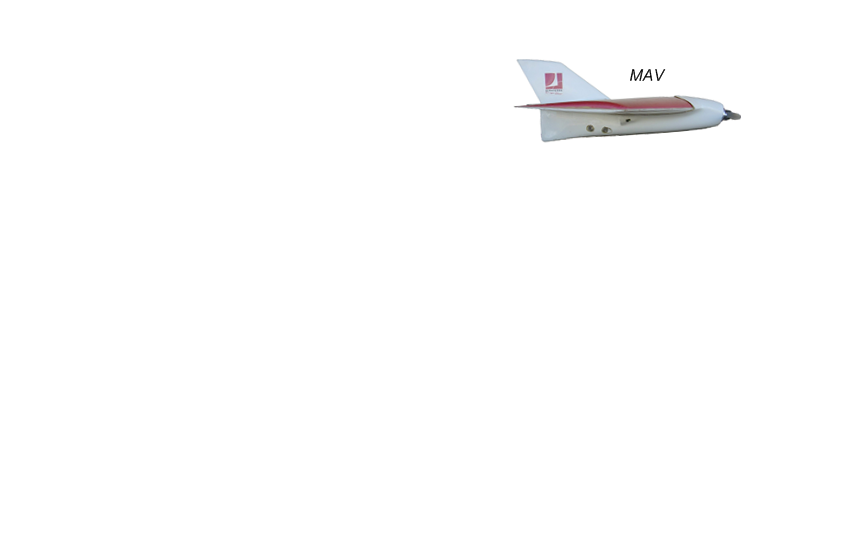
\includegraphics[height=6cm]{system/system_overview_0}<1>
    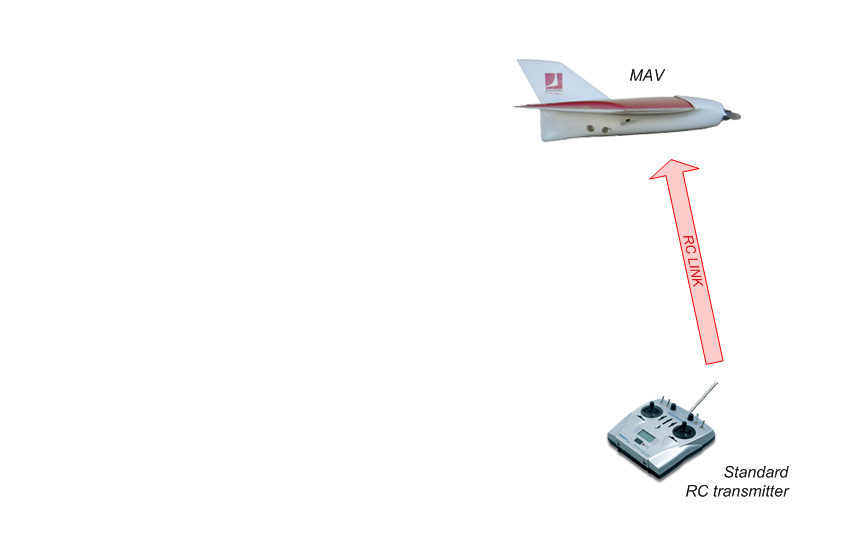
\includegraphics[height=6cm]{system/system_overview_1}<2>
    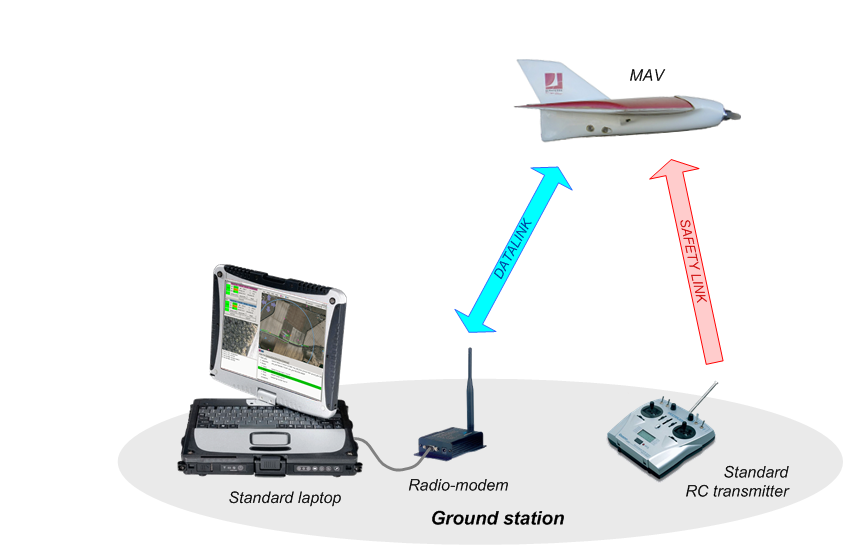
\includegraphics[height=6cm]{system/system_overview_2}<3>
    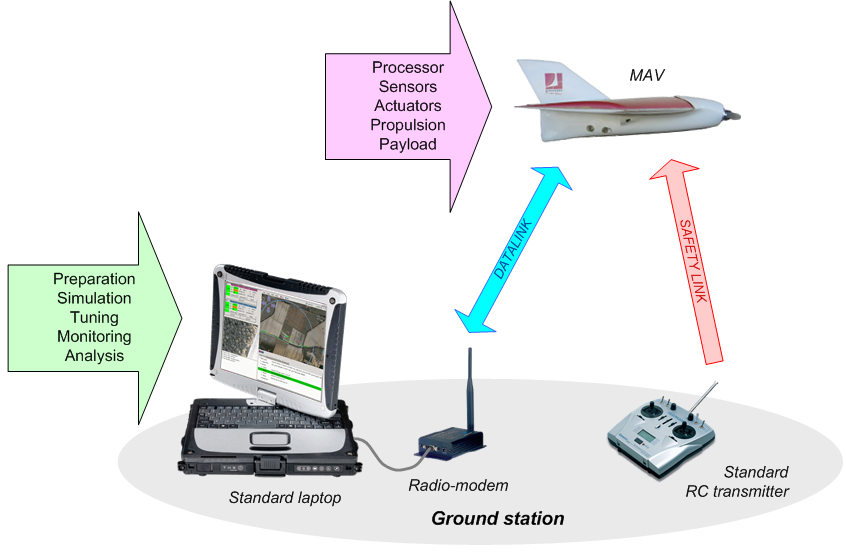
\includegraphics[height=6cm]{system/system_overview_3}<4>
  \end{center}
\end{frame}


%
% Features
%
\subsection{Features}


%
% History
%
\subsection{History}

%
%
% Flight demo
%
%
%

%
% Hardware
%
\subsection{Hardware}

%
% Software
%
\subsection{Software}

%
% Results
%
\subsection{Results}





\frame{} % to enforce entries in the table of contents

\end{document}
